\subsubsection{Lavpasfilter} \label{sec:lavpas_test}
For at undersøge, hvilken betydning det digitalt filtrede signal har i forhold til det samplede signal, visualiseres disse. De samplede signaler er fra pilotforsøget, som er beskrevet i \autoref{sec:pilotforsoeg}. Signalerne sendes til mikrokontrollen via en UART-forbindelse, hvorved den filtrede værdi returners og visualisers i MATLAB. Dette fremgår af \autoref{fig:lavpas_imp}.

\begin{figure}[H]
\centering
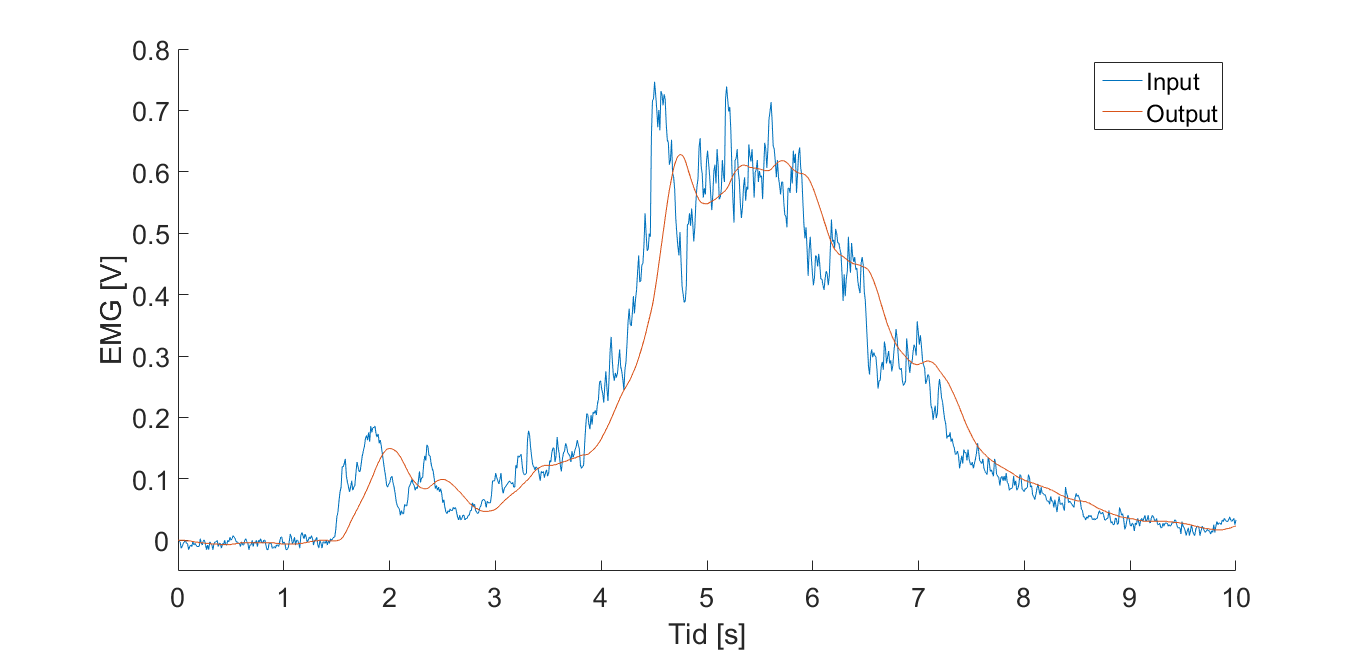
\includegraphics[width=1\textwidth]{figures/EMG_test}
\caption{Den blå graf illustrerer et samplet muskelsignal og den røde graf illustrerer et samplet filtrede muskelsignal.}
\label{fig:lavpas_imp}
\end{figure}

\noindent
Figuren illustrerer, at inputsignalet følger det samplede signal dog med forsinkelse. For at teste forsinkelsen i det filteret eksekveres, defineres en debug-pin. Denne pin sættes høj før funktionskaldet og lav efter funktionskaldet. For at måle, hvor længe pinen er høj, tilsluttes et oscilloskop. Ud fra dette kan der aflæses en forsinkelse på $175~\mu~s$, hvilket er den forsinkelse der går før data har passeret det digitale filter. Denne forsinkelse vurderes ikke at have nogen signifikant betydning.

For at vurdere om filteret dæmper nok i forhold til de opstillede krav i \autoref{sec:lavpas_krav}, udføres en test hvor forskellige frekvenser sendes gennem filteret. Hertil anvendes en funktionsgenerator, til at genererer et signussignaler mellem $0,5-20~Hz$. Disse frekvenser er valgt for at teste dæmpningen i passbåndet, og i transitionsbåndet.  
%Dette frekvensområde er valgt på baggrund af målinger fra \autoref{sec:pilotforsoeg}, hvor det fremgår, at signalet ligger mellem $0,4-10~Hz$.  
%Da funktionsgeneratoren ikke kan indstilles til en frekvens på $0~Hz$ indstilles denne til $1~\mu~Hz$. 
Amplituden af sinussignalet sættes til 1 $V_{pp}$ med et offset på $1,65~V$, da dette fortages ved single ended måling, hvortil sinussignalet ikke kan svinge omkring $0~V$. Yderligere tilsluttes et oscilloscope til funktionsgeneratoren, for at kontrollere det generede signal. Heraf aflæses amplituden til $1,08~V$.  
For at omregne det konverteret filtreret signal til en spænding, gangs de samplede værdier med LSB for ADC'en. 
Da amplituden for ingangssignalet og det filtreret signal kendes, anvendes \autoref{eq:deampning_db} til at udregne en dæmpning i dB.

\begin{equation}\label{eq:deampning_dB}
	dB = 20*log10(\frac{V_{in}}{V_{out}})
\end{equation}

\noindent
Dæmpningen for de forskellige frekvenser, fremgår af {fig:bodeplot}.

\begin{figure}[H]
\centering
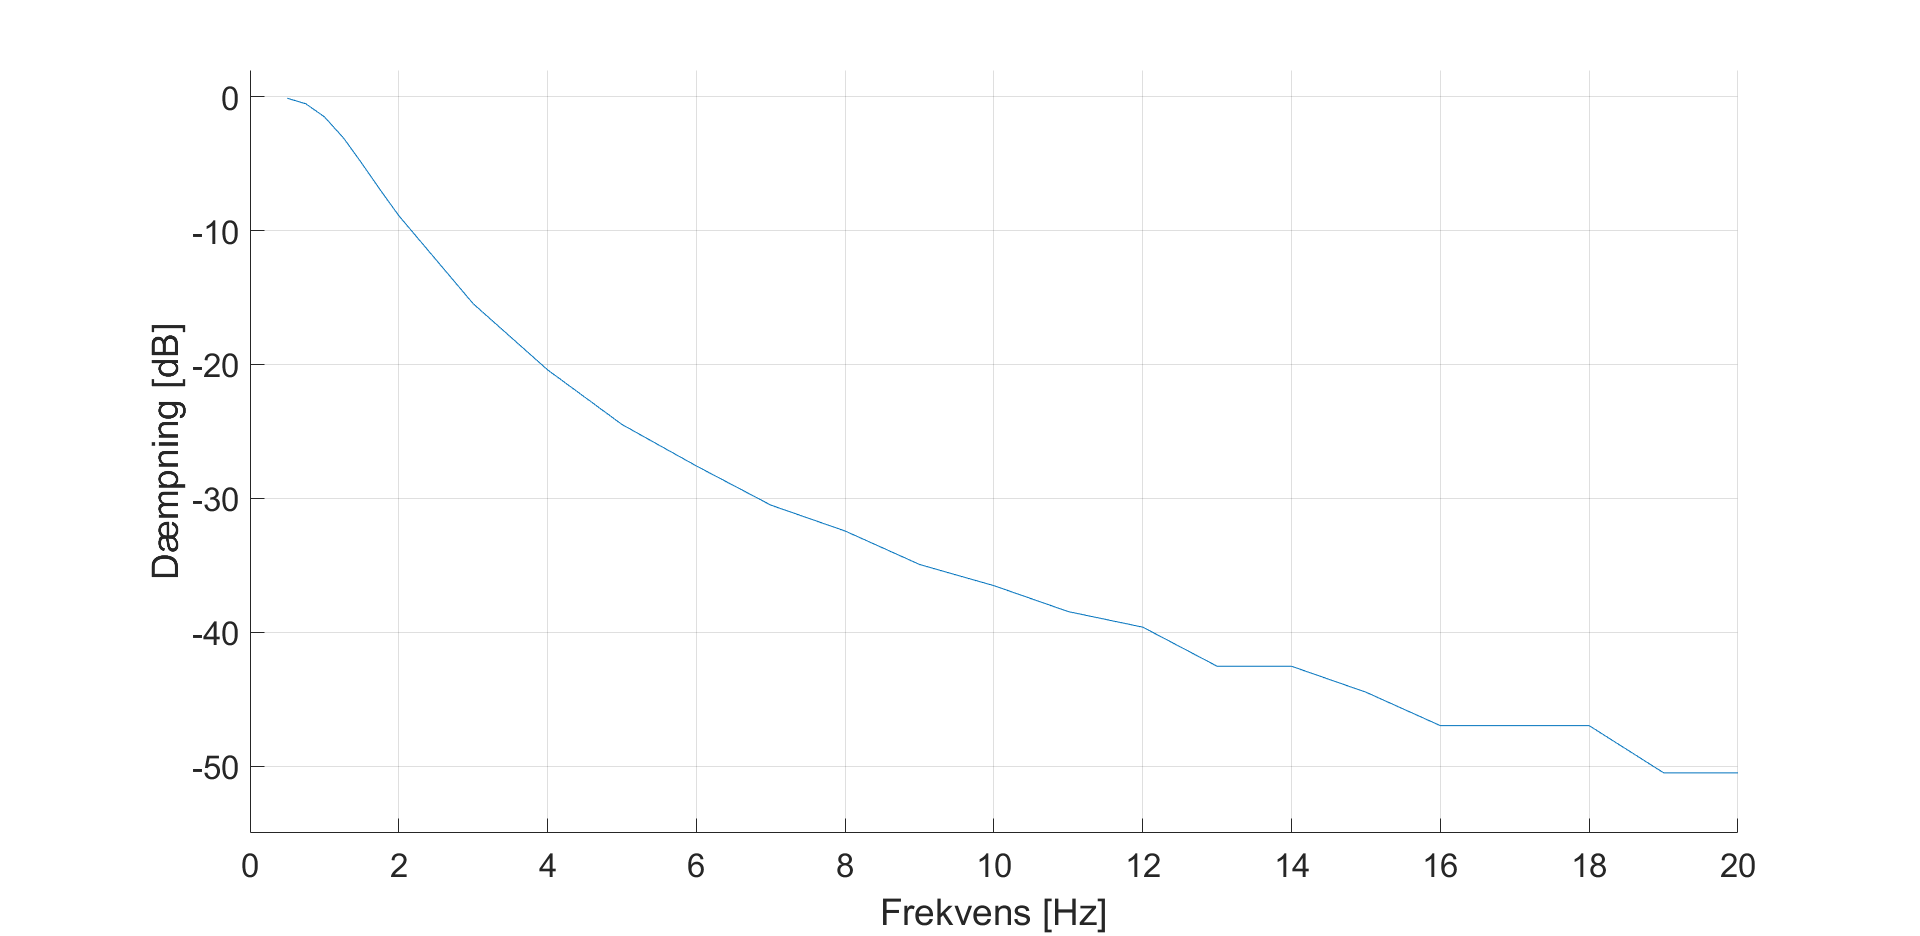
\includegraphics[width=0.8\textwidth]{figures/bodeplot_lavpas2}
\caption{Hertil ses bodeplottet for lavpasfilteret. Heraf fremgår dæmpningen ved forskellige frekvenser idet de passere lavpasfilteret.}
\label{fig:bodeplot}
\end{figure}

\noindent
Yderligere testes dæmpningen for knækfrekvensen, der forvestes at være $3~dB$. Resultatet heraf viser en dæmpning på $3,1~dB$ ved en frekvens på $1,26~Hz$ Dette stemmer overens med butterworth filter typen, hvortil afvigelsen på $0,1~dB$ ikke antages som værende af signifikant betydning i forhold til systemet virkemåde. 
På baggrund af de udførte test godtages filteret. 

%\noindent
%En dæmpning på $-3~dB$ for den valgte knækfrekvens på $1,26~Hz$ bestemmes, samt en dekade længere ude svarende til en frekvens på $50~Hz$. Da der anvendes et 2. ordens filter, skal denne frekvens dæmpes ved $-40~dB$. Da der er anvendt EMG-forstærkeren fremgår $50~Hz$ ikke, hvilket er beskrevet i \autoref{sec:EMG_imp}. Outputspændingen ved dennee dæmpningsfaktor er udregnet ved \autoref{equ:daempning1}. 
%
%\begin{equation} \label{equ:daempning1}
%-3~dB = 20 \cdot log_{10} \cdot (\frac{V_{out}}{1}) \Rightarrow V_{out} = 0,7 V
%\end{equation}
%
%\noindent
%Da det ikke er muligt at aflæse nøjagtige værdier for Vpp tages der udgangspunkt i de nærmeste værdi. Værdien for $1,26~Hz$ er  aflæst til $0,06~V$. Afvigelsen fremgår af \autoref{equ:afvigelse1}.
%%Da målingerne for $V_{pp}$ ikke er muligt at aflæse nøjagtige værdier, hvorfor der tages udgangspunkt i de nærmeste værdier. Værdierne for $5~Hz$ er $0,06~V$. Afvigelsen fremgår af \autoref{equ:afvigelse1}.
%
%\begin{equation} \label{equ:afvigelse1}
%Afviglese_{5~Hz} = \frac{0,06V-0,7V}{0,7V} \cdot 100\%  = - 14 \%
%\end{equation}
%
%\noindent 
%Afvigelserne for $1,26~Hz$ er 14\%. Dette betyder at filteret ikke dæmper signalet nok. Da målingerne for outputspændingen, målt ved de forskellige frekvenser, ikke er nøjagtig aflæst er det forventet, at der er en større afvigelse fra værdierne udregnet i \autoref{equ:daempning1}. På baggrund af dette godtages filteret. 

\vspace{3mm}
\textbf{Opsummering af krav:}
\begin{itemize}
\item[\text{\sffamily \checkmark}] Skal følge inputsignalet mest muligt  
\item[\text{\sffamily \checkmark}] Skal udformes som et Butterworth lavpasfilter
\item[\text{\sffamily \checkmark}] Skal have en knækfrekvens på $1,26~Hz$
\item[\text{\sffamily \checkmark}] Skal have en filterorden på 2
\end{itemize}